\subsection{How Developers Drive Software Evolution\\ \textit{T. Girba, A. Kuhn, M. Seeberger, S. Ducasse (IWPSE'2005)}}

The evolution of a project may sometimes be surprisingly fast, and developer knowledge becomes more and more important as the projects becomes more and more complex. Therefore it may sometimes be useful to know which developer might have the best knowledge of each file in the project in order to assign tasks such as bugfixes, or even to ask for help on the matter.
This paper defines the \emph{ownership} metric, as the degree to which a developer is the \emph{owner} of a file at a given time during the project's development\cite{Girba2005}.

In order to achieve this, they use the CVS logs of a project in order to calculate a number of metrics, and determine which developer might be considered as most knowledgeable of a file in the project, and designate him as \emph{owner} of that file.
They also created the following visualisation of ownership during a project's lifetime:

\begin{figure}[H]
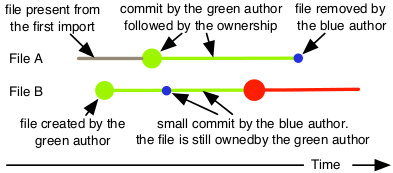
\includegraphics[keepaspectratio=true,scale=0.5]{./resources/girba2005.png}~
\caption{commit map}
\label{fig:commit_map}
\end{figure}

When this visualisation is applied to an entire project, it becomes possible to detect behavioural pattern between developers. See appendix[1].

Given that CVS is a file-based versionning system, a developer will be considered an owner of a file if he has written/edited the highest amount of lines within that file. This leaves the system open to inappropriate changes of ownership if for instance a developer decides to reformat the code, leading to a file owner who actually has little knowledge of the file.

On the other hand, this visualisation did allow them to detect behavioural patterns among the developers of projects:
\begin{itemize}
\itemsep-0.6em
\item \textbf{Monologue:} One developer is the owner of a portion of the project for a time.
\item \textbf{Dialogue:} Two or more developerss take ownership alternatively of a portion of the project.
\item \textbf{Teamwork:} Similar to Dialogue, with a quick succession of commits by several developers.
\item \textbf{Silence:} Little to no activity during a period.
\item \textbf{Takeover:} A developer suddenly takes ownership on a large portion of the project.
\item \textbf{Familiarisation:} Similar to a Takeover, but over a longer period of time.
\item \textbf{Expansion:} A Takeover followed by the addition of files to the project.
\item \textbf{Cleanup:} The opposite of Expansion, a developer deletes files or lines of code.
\item \textbf{Bugfix:} A small punctual change.
\item \textbf{Edit:} Non-functionnal changes (formatting, comments, ect...)
\end{itemize}

With these events, we can determine how the project was developed, who was the main developer, and more.